% \begin{document}

\chapter{Gestione Memoria}

Prima di discutere su i diversi modi in cui la memoria (RAM e HD solo se necessario) puo' essere gestita dal compilatore di un linguaggio, e' importante identificare cosa esattamente deve essere contenuto all'interno di essa. 

Sicuramente, ogni \textit{dato} che deve essere salvato durante l'esecuzione del programma dovra' avere un posto nella memoria, come ad esempio le variabili, ma ci sono anche informazioni per il \textit{controllo dell'esecuzione} che necessitano di essere memorizzati.

La vita di un oggetto corrisponde con tre meccanismi di allocazione di memoria:
\begin{itemize}
\item \textbf{Allocazione statica}: l'oggetto viene allocato una volta sola, prima dell'inizio dell'esecuzione del programma, e deallocato alla fine dell'esecuzione, 

\textit{pertanto è una memoria allocata a tempo di compilazione}
\item \textbf{Allocazione automatica}: l'oggetto viene allocato all'entrata di un blocco (tipicamente una funzione) e deallocato all'uscita del blocco.


\item \textbf{Allocazione dinamica}: l'oggetto viene allocato e deallocato esplicitamente dal programmatore tramite chiamate a funzioni di allocazione e deallocazione (ad esempio, \texttt{malloc} e \texttt{free} in C).
\textit{pertanto è una memoria allocata a tempo di esecuzione}

Questo tipo di allocazione di serve di due aree di memoria:
\begin{itemize}
  \item pila (stack): gli oggetti sono allocati con una politica LIFO, utilizzato per le variabili locali e i parametri formali delle funzioni
  \item heap: gli oggetti sono allocati e deallocati in qualsiasi ordine, utilizzato per gli oggetti dinamici (puntatori)
  \end{itemize}
\end{itemize}

\section{Allocazione Statica}
Non sarebbe possibile utilizzare solo una memoria con allocazione statica? Sicuramente per le variabili \textit{globali}, \textit{costanti} che non dipendono da altri valori non noti inizialmente e anche per le \textit{tabelle} che utilizza il compiler, l'allocazione statica funziona benissimo. 

Per quanto riguarda i sottoprogrammi, si puo' pensare di allocare per ognuna di esse tutto lo spazio necessario per i parametri e le variabili locali (e altre informazioni necessarie), dato che possiamo determinare tutto cio' prima di eseguire il programma:
\begin{center}
  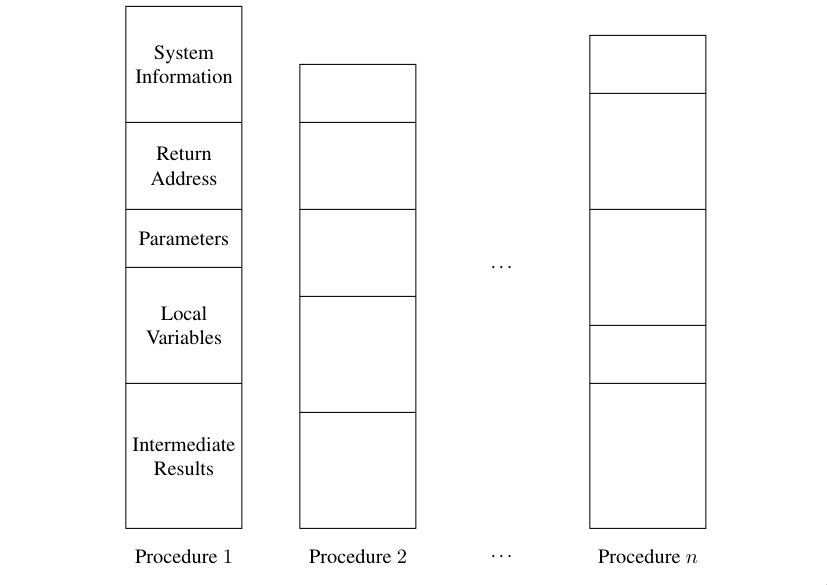
\includegraphics[width=0.5\textwidth]{img/2025-03-02-10-46-16.png}
\end{center}

Questo metodo funziona solo se siamo sicuri che, se una procedura e' attiva, allora non puo' chiamare la stessa procedura ricorsivamente. Questo e' perche' esiste solo un'istanza per ogni procedura allocata in memoria e non e' possibile sapere quante volte una funzione verra' chiamata ricorsivamente. Quindi, se vogliamo implementare la ricorsione, serve l'allocazione \textit{dinamica} (stack di chiamate):

\section{Allocazione Dinamica}
\subsection{Allocazione Dinamica con Pila}

Ogni istanza di sottoprogramma viene memorizzata con un \textit{frame} (o \textit{record di attivazione}) che contiene tutte le informazioni necessarie. Quando un'istanza viene attivata, il relativo frame viene messo in cima a una \textbf{pila}, la struttura dati naturale in quanto se una procedura A chiama una procedura B, allora siamo sicuri che B deve terminare prima che A possa continuare l'esecuzione e terminare anch'esso.

\nt{
  L'allocazione dinamica e' utile anche quando non c'e' ricorsione come meccanismo per risparmiare memoria.
}

Vediamo un esempio:

\begin{lstlisting}[language=C]
  A:{int x = 0;
    void pippo(int n){
      x = n+1;
    }
    pippo(3);
    write(x);
    {
      int x = 0;
      pippo(3);
      write(x);
    }
    write(x);
  }
\end{lstlisting}

\begin{center}
  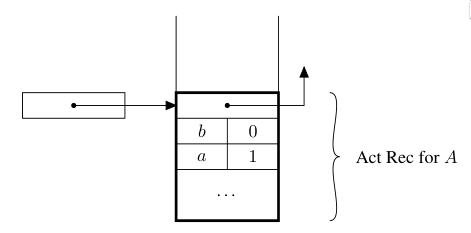
\includegraphics[width=0.3\textwidth]{img/2025-03-02-11-40-29.png}
  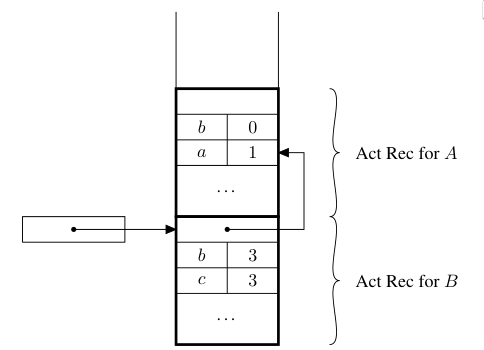
\includegraphics[width=0.3\textwidth]{img/2025-03-02-11-41-09.png}
  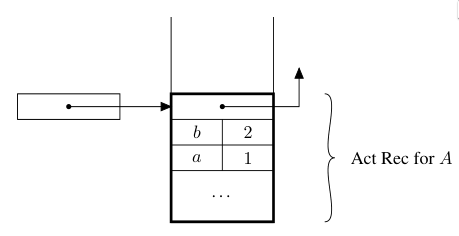
\includegraphics[width=0.3\textwidth]{img/2025-03-02-11-42-23.png}
\end{center}

Vediamo piu' in dettaglio cosa viene memorizzato nei record di attivazione:

\subsubsection{Record di attivazione}
Per un semplice blocco anonimo, il corrispondente frame ha tale forma:
\begin{center}
    \renewcommand{\arraystretch}{2} % Increase row height
    \setlength{\tabcolsep}{2em} % Adjust column spacing
    
    \begin{tabular}{|c|}
        \hline
        \textbf{Dynamic chain pointer} \\ \hline
        \textbf{Local variables} \\ \hline
        \textbf{Intermediate results} \\ \hline
    \end{tabular}
\end{center}

\nt{
  Nella realta' la maggior parte dei linguaggi usa l'allocazione statica per blocchi anonimi per maggiore efficenza di calcolo (sacrificando pero' l'efficenza di memoria).
}

Mentre per le procedure e' un po' piu' complesso:
\begin{center}
    \renewcommand{\arraystretch}{1.8} % Increase row height for better spacing
    \setlength{\tabcolsep}{2em} % Adjust column spacing
    
    \begin{tabular}{|c|}
        \hline
        \textbf{Dynamic Chain Pointer} \\ \hline
        \textbf{Static Chain Pointer} \\ \hline
        \textbf{Return Address} \\ \hline
        \textbf{Address for Result} \\ \hline
        \textbf{Parameters} \\ \hline
        \textbf{Local Variables} \\ \hline
        \textbf{Intermediate Results} \\ \hline
    \end{tabular}
\end{center}

Vediamo in dettaglio cosa sono tutti sti dati:
\begin{itemize}
\item \textbf{Intermediate Results}: serve per memorizzare risultati intermedi di equazioni complicate e per risultati di chiamate ricorsive.
\item \textbf{Local Variables} e \textbf{Parameters}: per le variabili locali e parametri.
\item \textbf{Dynamic Chain Pointer}: puntatore all'ultimo RdA creato sulla stack, l'insieme di tutti i puntatori dinamici e' chiamata \textit{catena dinamica}.
\item \textbf{Static Chain Pointer}: informazione necessaria per implementare lo scope statico, vedremo piu' avanti.
\item \textbf{Return Address}: indirizzo di memoria della prima istruzione da eseguire quando termina la procedura corrente.
\item \textbf{Address for Result}: indirizzo dove puo' essere salvato il valore di ritorno della funzione (sara' un indirizzo interno al frame della funzione chiamante).
\end{itemize}

\subsubsection{Gestione della Pila}

Vediamo la struttura di un sistema a pila (discendente):
\begin{center}
  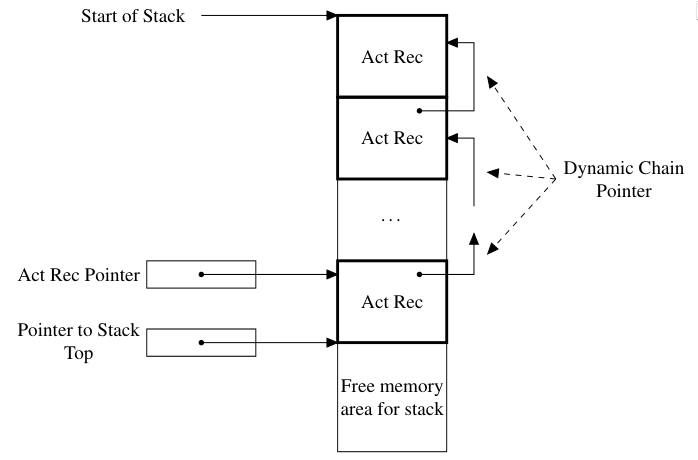
\includegraphics[width=0.5\textwidth]{img/2025-03-02-12-39-06.png}
\end{center}

Come puo' notare dall'immagine, ci sono due puntatori esterni che puntano a posti specifici sull'ultimo record di attivazione:
\begin{itemize}
  \item \textbf{Pointer al RdA}: e' un puntatore ad un luogo predeterminato all'interno del frame usato come base da cui si puo' calcolare l'offset per accedere alle variabili locali. Questo offset e' determinabile staticamente dal compilatore (ad eccezzione del caso di variaili di dimensione variabile).
\item \textbf{Stack Top Pointer}: come si puo' indovinare, e' il puntatore al primo indirizzo libero di memoria dopo l'ultimo RdA. Puo' essere omesso se e' possibile calcolare lo stesso indirizzo partendo dal pointer al RdA.
\end{itemize}

Il funzionamento corretto della pila di RdA e' dato dalla collaborazione fra il chiamante e il blocco chiamato, che eseguono dei blocchi di codice inseriti dal compilatore (o interprete) prima e dopo chiamate a procedure e blocchi anonimi:
\begin{itemize}
\item \textbf{Sequenza di Chiamata}: eseguito dal chiamante subito prima della chiamata
\item \textbf{Prologo}: eseguito immediatamente all'inizio del blocco chiamato
\item \textbf{Epilogo}: eseguito alla fine del blocco
\item \textbf{Sequenza di Ritorno}: eseguito dal chiamante immediatamente dopo la chiamata
\end{itemize}

Al momento della chiamata, la Sequenza di Chiamata e il Prologo devono:
\begin{itemize}
\item \textbf{Modificare PC}
\item \textbf{Allocare spazio sulla pila}
\item \textbf{Modifica pointer RdA}
\item \textbf{Passaggio parametri}
\item \textbf{Memorizzare registri}
\end{itemize}

Quado il blocco o processo chiamato termina, l'Epilogo e la Sequenza di Ritorno devono:
\begin{itemize}
\item \textbf{Modificare PC}
\item \textbf{Ritornare Valori}
\item \textbf{Recuperare Registri}
\item \textbf{Deallocare spazio sulla pila}
\end{itemize}

\nt{
  Sono stati omessi meccanismi per l'implementazione delle regole di scope. Vedremo queste piu' avanti.
}

\subsection{Allocazione Dinamica con Heap}

Nel caso in cui vogliamo dare la possibilita' a chi usa il linguaggio di allocare esplicitamente memoria a run-time o di usare oggetti di dimensioni variabili sorge il seguente problema: la vita degli oggetti non e' per forza LIFO, ovvero un oggetto creato prima di un altro puo' essere rimosso dalla memoria prima di un'altro oggetto creato dopo, come nel seguente blocco di codice:

\begin{lstlisting}[language=C]
  int *p, *q;
  p = malloc(sizeof(int));
  q = malloc(sizeof(int));
  *p = 0;
  *q = 1;
  free(p);
  free(q);
\end{lstlisting}

Dobbiamo usare quindi la \textit{heap}, ovvero una regione di memoria i cui blocchi possono essere allocati/deallocati in momenti arbitrari.

\nt{
  La heap che abbiamo appena definito non centra niente con la struttura dati usata per la "heap sort".
}

Esistono due categorie principali di metodi di gestione della heap a seconda della lunghezza dei blocchi che memorizza, che possono essere di \textit{dimensione fissa} o \textit{variabile}.

\subsubsection{Dimensione fissa}

La heap viene suddivisa in blocchi di dimensione fissa abbastanza limitata che sono inizialmente collegati tutti assieme nella \textit{lista libera}:
\begin{center}
  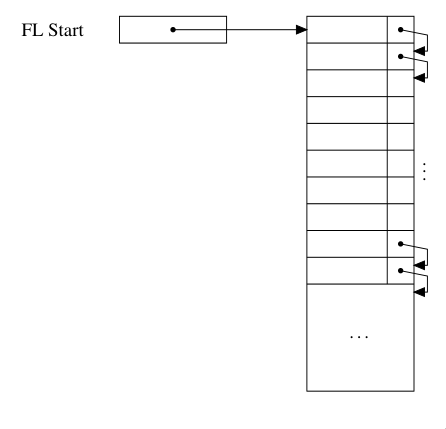
\includegraphics[width=0.3\textwidth]{img/2025-03-02-15-29-56.png}
\end{center}

A run-time, quando viene richiesto un blocco di memoria, il primo elemento della lista libera viene rimosso e restituito al processo che ha richiesto la memoria, mentre la testa della lista libera si sposta al prossimo elemento della lista. Vediamo un esempio di heap a dimensione fissa dopo alcune operazioni di allocazione/deallocazione (i blocchi grigi sono in uso):
\begin{center}
  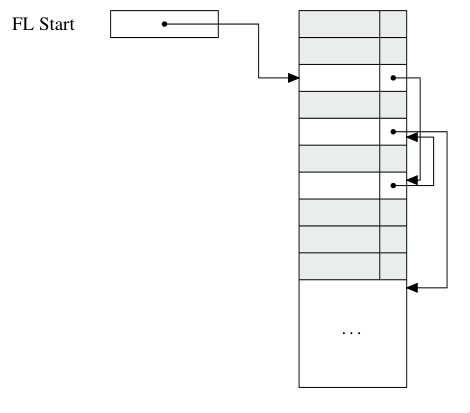
\includegraphics[width=0.3\textwidth]{img/2025-03-02-15-32-35.png}
\end{center}

\subsubsection{Dimensione variabile}

Nel caso volessimo poter allocare array la cui dimensione e' determinata solo a runtime, la soluzione a dimensione fissa non sarebbe adeguata, dato che l'array puo' essere di dimensioni maggiori rispetto ai blocchi fissi e non si possono allocare piu' blocchi perche' la memoria deve essere per forza contigua. 

In questi casi e' necessario poter richiedere un blocco di dimensione arbitraria. In un sistema di questo tipo, bisogna prestare attenzione ad usare \textit{operazioni efficenti} e a limitare lo \textit{spreco di memoria} che puo' avvenire in due situazioni:
\begin{itemize}
\item \textbf{Frammentazione interna}: viene richiesto un blocco di dimensione $ n $ ma ne viene restituito uno di dimensione $ k > n $, quindi $ k-n $ parole si perdono.
\item \textbf{Frammentazione esterna}: lo spazio totale nella memoria sarebbe abbastanza per soddisfare una richista di dimensione $ n $, ma i blocchi liberi sono separati o non contigui.
  \begin{center}
    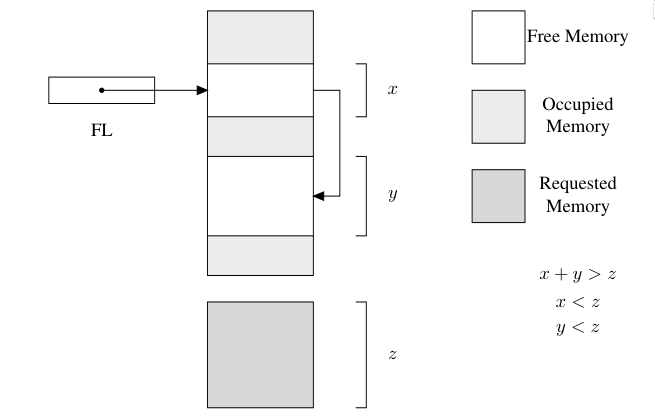
\includegraphics[width=0.4\textwidth]{img/2025-03-02-16-01-30.png}
  \end{center}
\end{itemize}

Esistono due meccanismi diversi per gestire blocchi di dimensione variabile:
\begin{itemize}
\item \textbf{Unica lista}: 

  Inizialmente, la lista libera e' composta da un solo blocco che occupa tutta la heap. Quando viene fatta la richiesta per un blocco di dimensione $ n $, le prime $ n $ parole dell'heap vengono allocate e l'inizio della lista si sposta di $ n $. Si va avanti cosi' finche' la memoria rimasta dall'inizio della lista libera alla fine della heap non e' abbastanza per soddisfare la richiesta. In queslto caso dobbiamo riutilizzare memoria deallocata, che puo' essere fatto in due modi:
    \begin{itemize}
      \item \textbf{Uso diretto della lista libera}: si scorre lungo la lista finche' si trova un blocco di dimensioni $ k > n $. Se la differenza fra la grandezza del blocco e della memoria effettivamente usata e' maggiore di una tolleranza, allora il blocco viene diviso ed il blocco di dimensione $ k - n $ viene reinserito nella lista. Possono essere usate due politiche di ricerca diverse per scegliere quale blocco prendere: \textit{first fit} e \textit{best fit}. Quando un blocco viene deallocato, si guarda se blocchi adiacenti sono anch'essi liberi e in caso affermativo si fondono per formare un blocco piu' grande (\textit{compattazione parziale}).
      \item \textbf{Compattazione della memoria libera}: tutti i blocchi attivi vengono spostati alla fine della heap, molto efficente ma funziona solo quando possiamo spostare la memoria.
    \end{itemize}
  \item \textbf{Liste libere Multiple}:

    Per ridurre il costo operativo di cercare un blocco di dimensione arbitraria, e' possibile utilizzare diverse liste per diverse dimensioni di blocchi. Quando viene richiesto un blocco di dimensione $ n $, si scorrono le liste finche' una che contiene blocchi di dimensioni adeguate non e' vuota. Anche in questo caso e' possibile riudurre la dimensione dei blocchi per ridurre la frammentazione interna, esistono due metodi:
    \begin{itemize}
      \item \textbf{Buddy system}: la dimensione dei blocchi aumenta per potenze di 2. Si calcola l'intero minore $ k $ tale che $ 2^k \geq n $ e si controlla se la relativa lista ha blocchi liberi. Altrimenti, si va a cercare nella lista $ k+1 $ e si divide il blocco in due blocchi da $ 2^k $ (la dimensione che volevamo), uno viene allocato e l'altro viene spostato nella lista corretta. Quando viene deallocato, la meta' cerca il suo compagno nella lista libera e se lo trova si uniscono e tornano nella lista originale.
      \item \textbf{Fibonacci}: funzionamento equivalente ma le dimensioni dei blocchi seguono la sequenza di Fibonacci, che sale piu' lentamente quindi porta a meno frammentazione ma piu' tempo.
    \end{itemize}
\end{itemize}

TODO: disegni esplicativi

% \end{document}
